
\section{How Do DANs Work?}
\label{sec:discussion}

In this section we first examine how the deep layers of the \dan\ amplify tiny
differences in the vector average that are predictive of the output
labels. Next, we compare \dan s to \drnn s on sentences that contain negations
and contrastive conjunctions and find that both models make similar errors
despite the latter's increased complexity. Finally, we analyze the predictive
ability of unsupervised word embeddings on a simple sentiment task in an effort
to explain why initialization with these embeddings improves the \dan.




\begin{figure}[t!]
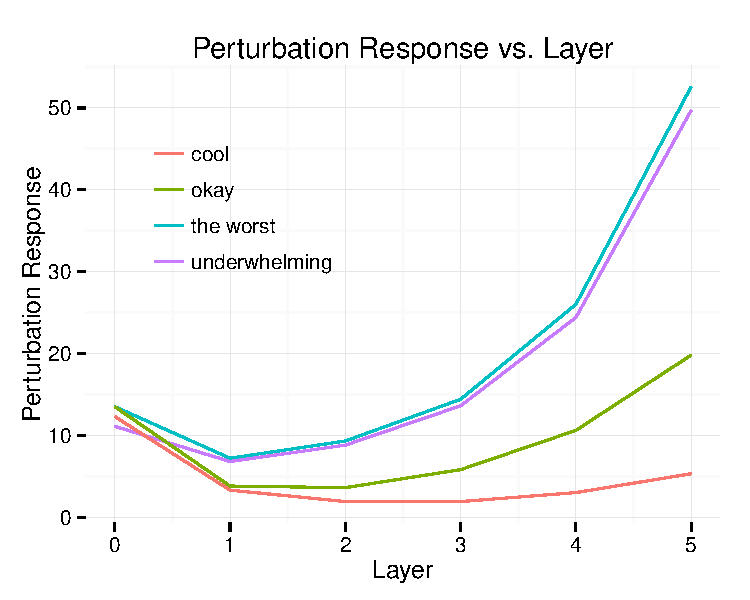
\includegraphics[scale=0.6]{2015_acl_dan/figures/perturb_2.pdf}
  \caption{Perturbation response (difference in 1-norm) at each layer of a 5-layer \dan\ after replacing \emph{awesome} in \emph{the film's performances were awesome} with four words of varying sentiment polarity. While the shallow \nbow\ model does not show any meaningful distinctions, we see that as the network gets deeper, negative sentences are increasingly different from the original positive sentence.}
\label{fig:perturb}

\end{figure}

\begin{figure}[t!]
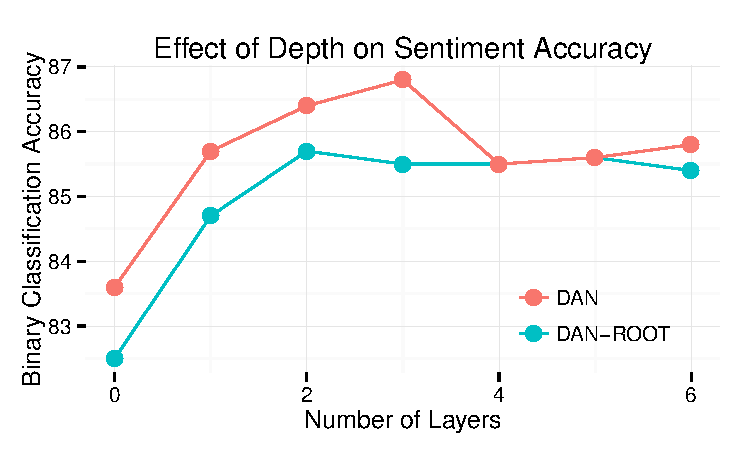
\includegraphics[scale=0.6]{2015_acl_dan/figures/layers.pdf}
  \caption{Two to three layers is optimal for the \dan\ on the \abr{sst} binary sentiment
          analysis task, but adding any depth at all is an improvement over the
          shallow \nbow\ model.}
\label{fig:slayers}
\end{figure}









\subsection{Perturbation Analysis}

Following the work of \newcite{irsoy-drsv}, we examine our network by measuring
the response at each hidden layer to perturbations in an input sentence. In
particular, we use the template \emph{the film's performances were awesome} and
replace the final word with increasingly negative polarity words (\emph{cool},
\emph{okay}, \emph{underwhelming}, \emph{the worst}). For each perturbed
sentence, we observe how much the hidden layers differ from those associated
with the original template in 1-norm.

Figure~\ref{fig:perturb} shows that as a \dan\ gets deeper, the differences
between negative and positive sentences become increasingly amplified. While
nonexistent in the shallow \nbow\ model, these differences are visible even with
just a single hidden layer, thus explaining why deepening the \nbow\ improves
sentiment analysis as shown in Figure~\ref{fig:slayers}.

\begin{table*}[ht]
  \begin{center}
    \begin{tabular}{p{8cm}ccc}
    \toprule
    Sentence & \dan & \drnn & Ground Truth \\
    \midrule
  \footnotesize
    a \hemph{lousy}  movie that's \hemph{not} merely \hemph{unwatchable}, but also \hemph{unlistenable} & \hemph{negative} & \hemph{negative} & \hemph{negative}\\
    \footnotesize
  if you're \hemph{not} a \kemph{prepubescent} \eemph{girl}, you'll be \aemph{laughing} at \hemph{britney} \hemph{spears}' \eemph{movie-starring} \eemph{debut} whenever it does \hemph{n't} have you \kemph{impatiently} \hemph{squinting} at your \eemph{watch} & \kemph{negative} & \kemph{negative} & \kemph{negative} \\
    \footnotesize
  \aemph{blessed} with \aemph{immense} \aemph{physical} \aemph{prowess} he \kemph{may} well be, but \hemph{ahola} is \eemph{simply} \hemph{not} an \eemph{actor} & \eemph{positive} & neutral & \kemph{negative}\\
    \footnotesize
  who \aemph{knows} what \kemph{exactly} \kemph{godard} is on about in this \eemph{film}, but his \aemph{words} and images do \hemph{n't} have to \aemph{add} up to \aemph{mesmerize} you. & \eemph{positive} & \eemph{positive} & \eemph{positive}\\
    \footnotesize
  it's so \aemph{good} that its \kemph{relentless}, \aemph{polished} \eemph{wit} can \eemph{withstand} \hemph{not} \kemph{only} \hemph{inept} school \aemph{productions}, but even \aemph{oliver} \aemph{parker}'s movie \eemph{adaptation} & \kemph{negative} & \eemph{positive} & \eemph{positive}\\
    \footnotesize
  \kemph{too} \hemph{bad}, but \aemph{thanks} to some \aemph{lovely} \aemph{comedic} \eemph{moments} and several \aemph{fine} \eemph{performances}, it's \hemph{not} a \hemph{total} \hemph{loss} & \kemph{negative} & \kemph{negative} & \eemph{positive}\\
  \midrule
    \footnotesize
  this movie was \hemph{not} \aemph{good} & \kemph{negative} & \kemph{negative} & negative\\
    \footnotesize
  this movie was \aemph{good} & \aemph{positive} & \aemph{positive} & positive\\
    \footnotesize
  this movie was \hemph{bad} & \hemph{negative} & \kemph{negative} & negative\\
    \footnotesize
  the movie was \hemph{not} \hemph{bad} & \hemph{negative} & \kemph{negative} & positive\\
    \bottomrule
    \end{tabular}
    \end{center}
  \caption{Predictions of \dan\ and \drnn\ models on real (top) and synthetic
    (bottom) sentences that contain negations and contrastive conjunctions. In
    the first column, words colored red individually predict the negative label
    when fed to a \dan, while blue words predict positive. The \dan\ learns that
    the negators \emph{not} and \emph{n't} are strong negative predictors, which
    means it is unable to capture double negation as in the last real example
    and the last synthetic example. The \drnn\ does slightly better on the synthetic
    double negation, predicting a lower negative polarity.}

\label{table:examples}
\end{table*}


\subsection{Handling Negations and ``but'': Where Syntax is Still Needed }

While \dan s outperform other bag-of-words models, how can they model linguistic
phenomena such as negation without considering word order? To evaluate \dan s
over tougher inputs, we collect 92 sentences, each of which contains at least one
negation and one contrastive conjunction, from the dev and test sets of the
\abr{sst}.\footnote{We search for non-neutral sentences containing \emph{not} /
  \emph{n't}, and \emph{but}. 48 of the sentences are positive while 44 are
  negative.} Our fine-grained accuracy is \emph{higher} on this subset than on
the full dataset, improving almost five percent absolute accuracy to
53.3\%. The \drnn\ model of \newcite{irsoy-drsv} obtains a similar
accuracy of 51.1\%, contrary to our intuition that syntactic functions should
outperform unordered functions on sentences that clearly require syntax to
understand.\footnote{Both models are initialized with pretrained 300-d GloVe embeddings for fair comparison.}

Are these sentences truly difficult to classify? A close inspection reveals that
both the \dan\ and the \drnn\ have an overwhelming tendency to predict negative
sentiment (60.9\% and 55.4\% of the time for the \dan\ and \drnn\ respectively) when they see a negation compared
to positive sentiment (35.9\% for \dan s, 34.8\% for \drnn s). If we further
restrict our subset of sentences to only those with positive ground truth
labels, we find that while both models struggle, the \drnn\ obtains 41.7\% accuracy, outperforming the \dan's 37.5\%.

To understand why a negation or contrastive conjunction triggers a negative
sentiment prediction, we show six sentences from the negation subset and four
synthetic sentences in Table~\ref{table:examples}, along with both models'
predictions. The token-level predictions in the table (shown as colored boxes)
are computed by passing each token through the \dan\ as separate test
instances.  The tokens \emph{not} and \emph{n't} are strongly predictive of
negative sentiment. While this simplified ``negation'' works for many
sentences in the datasets we consider, it prevents the \dan\ from reasoning
about double negatives, as in ``this movie was not bad''. The \drnn\ does
slightly better in this case by predicting a lesser negative polarity than the
\dan; however, we theorize that still more powerful syntactic composition
functions (and more labelled instances of negation and related phenomena) are
necessary to truly solve this problem.

























\subsection{Unsupervised Embeddings Capture Sentiment}

Our model consistently converges slower to a worse solution (dropping 3\% in
absolute accuracy on coarse-grained \abr{sst}) when we randomly initialize the
word embeddings. This does not apply to just \dan s; both convolutional and
recursive networks do the same~\cite{kim:2014:EMNLP2014,irsoy-drsv}. Why are
initializations with these embeddings so crucial to obtaining good performance?
Is it possible that unsupervised training algorithms are already capturing
sentiment?

We investigate this theory by conducting a simple experiment: given a sentiment
lexicon containing both positive and negative words, we train a logistic
regression to discriminate between the associated word embeddings (without any
fine-tuning). We use the lexicon created by~\newcite{hu2004mining}, which
consists of 2,006 positive words and 4,783 negative words. We balance and split
the dataset into 3,000 training words and 1,000 test words. Using
300-dimensional \texttt{GloVe} embeddings pretrained over the Common Crawl, we
obtain over 95\% accuracy on the unseen test set, supporting the hypothesis that
unsupervised pretraining over large corpora can capture properties such as
sentiment.

Intuitively, after the embeddings are fine-tuned during \dan\ training, we might
expect a decrease in the norms of stopwords and an increase in the norms of
sentiment-rich words like ``awesome'' or ``horrible''. However, we find no
significant differences between the $L_2$ norms of stopwords and words in the
sentiment lexicon of~\newcite{hu2004mining}.
